\documentclass{article}
\usepackage{enumitem}
\usepackage{graphicx}
\usepackage{amsmath}
\graphicspath{{image/} }

\begin{document}
\begin{titlepage}
	\begin{center}
		\Huge
		\textbf{Travail Pratique 1}\\
		\textbf{Architecture du Processeur}\\

		\vspace{2.0cm}
		\Large
		\textbf{Julien Legault, 1847125} \\
		\textbf{Billy Bouchard, 1850477}

		\vspace{2.0cm}
		Inf1600 - Architecture des micro-ordinateur
		\vfill
		Un Travail pr\'esent\'e \`a :\\
		Abdellatif Amrani \\
		\vspace{1.0cm}
		Groupe B1

		\vspace{0.8cm}

		
\includegraphics[width=0.4\textwidth]{university.png}

		\Large
		D\'epartement G\'enie informatique et Logiciel\\
		Polytechnique Montreal\\
		le 28 spetembre 2017\\

	\end{center}
\end{titlepage}

\section*{Exercice 1}
\begin{enumerate}
	\item $00101010 = 42$
	\item On considere pour chacun d'entre eux que le premier bit est le bit de signe
	      \begin{enumerate}[label=\alph*)]
	      	\item $11110101 = -128+117 = -11$
	      	\item $4517 = 100101001111 =-2048+335 =-1713 $ ou sans bit de signe $4517 = 2383 $
	      	\item $CAFE = 1100101011111110 = -32768 +19198 = -13570$ ou sans bit de signe $CAFE = 51966$
	      	\item $10000000 = -128 $
	      \end{enumerate}
	\item
\end{enumerate}
\begin{minipage}{\linewidth}
	\centering
	\begin{tabular}{c | c | c | c | c | c }
		ID  & Num\'eros & BIN  & OCT  & DEC  & HEX  \\ \hline
		(a) & 5781      & faux & faux & vrai & vrai \\ \hline
		(b) & 10000000  & vrai & vrai & vrai & vrai \\ \hline
		(c) & 1600      & faux & vrai & vrai & vrai \\ \hline
		(d) & B747      & faux & faux & faux & vrai \\ \hline
		(e) & 00000000  & vrai & vrai & vrai & vrai \\
	\end{tabular}
\end{minipage}
\begin{enumerate}
	\setcounter{enumi}{2}
	\item
	      la solution prend 3 en binaire 0b11 et le bitshift de 4 de facon a obtenir 48
	      (0b110000). Ensuite, elle compare bit par bit 48 avec la valeur de x et l'affecte a la variable y
	\item
	      \begin{enumerate}[label=\alph*)]
	      	\item $-1234 = -32678 + 31534 = 0b1111101100101110 = 0xFB2E$
	      	\item $32767 =  0b00111111111111111 = 0x7FFF$
	      	\item $-32 =  -32678 + 32646 = 0b1111111110000110  = 0xFF86$
	      \end{enumerate}
	\item
	      \begin{enumerate}[label=\alph*)]
	      	\item $7C +4F = 0b01111100 + 0b01001111 = 0b10001011$ donc il y a un debordement sign\'ee
	      	      $ 0b10001011 = 0x8B$
	      	\item On prend pour aquis qu'ils sont en d\'ecimal :
	      	      $89 + 11 = 0b01011001 + 0b00001011 = 0b01100100 = 0x64$ aucun debordement
	      \end{enumerate}
	\item
	      \begin{enumerate}[label=\alph*)]
	      	\item si nous sommes en big-endian, les octets les plus significatif sont dans la plus petite addresse m\'emoire (soit $oct_2$) :\\
	      	      donc, on prend les 4 octets que repr\'esente le nombre 86 et on le traduit :  $0x86 = 134$ et nous avons la r\'eponse

	      	\item la version little-endian veut le contraire de big-endain dans le sens ou les bits les + significatif sont a la plus grande addresse m\'emoire :\\
	      	      donc, on prend plutot les 2 avant derniers chiffres soit EE que l'on convertit en octal pour voir les octets: $0xEE = 0o0356$ par la suite on inverse le nombre pour obtenir la valeur de chaque octet:
	      	      $0o6530 = 3416$

	      \end{enumerate}
\end{enumerate}

\newpage
\section*{Exercice 2}
\begin{enumerate}[label=\alph*)]
	\item Calculez l'espace total sur le disque dur. \\
	      espace total = tailleZone1 + tailleZone2 + tailleZone3 +tailleZone4 \\
	      tailleZone = Pistes/Zone x Secteurs/Piste x Octets/secteur = Octets/Zone \\
	      \begin{align*}
	      	tailleZone1  & = 624\times 792\times 512 = 235 034 496 B                 \\
	      	tailleZone2  & =1424\times 780\times 512 = 568 688 640 B                 \\
	      	tailleZone3  & =1680\times 760\times 512 = 653 721 600B                  \\
	      	tailleZone4  & =1815\times 720\times 512 = 669 081 600 B                 \\
	      	EspaceTotale & = 235 034 496 B + 568 688 640 B +
	      	653 721 600B +  669 081 600 B \\
	      	             & =  2 126 526 336 B                                        \\
	      	             & =  \frac {2 126 526 336 B}{2^{20}\frac{B}{MB}} =  2028 MB
	      \end{align*}
	\item Calculez le taux de lecture. \\
	      taux(b/s) =vitesse de rotation(T/s) x moyenneNbsecteurs/Piste(S/P) x octet/secteur(B/S) x bits/octet(b/B)
	      \begin{align*}
	      	taux ={ \frac{5400}{60}\times( 0,25\times792+0,25\times780+0,25\times760+0,25\times720)\times512\times8} \\
	      	= 281 272 320 b/s =  \frac {281 272 320}{2^{20}}= 268,24 Mb/s
	      \end{align*}
	\item Il n'est pas nécessaire d'effectuer ce calcul pusique le taux de lecture efficace du disque va être de 268,24 Mb/s  puisque ce taux est inférieur au taux de transfert du bus de 400mb/s. \\
	      d)Au niveau de l'espace total, oui, car plus de surface peremettrait plus de secteurs donc plus de place pour mettre des données. Par contre, au niveau du taux de lecture, le taux de lecture va rester le même puisque le nombre de surfaces n'influencent pas le temps nécessaire pour que le bras mécanique balaie les données puisqu'elles sont sur une même surface.
\end{enumerate}

\newpage
\section*{Exercice 3}
\begin{enumerate}
	\item SUBMUL Ra, Rb, k \\
	      \[(op = 5) \rightarrow	R[a]  \leftarrow k \times (R[a] - R[b]);\] \\
	\item DECREM Ra, Rb \\
	      \[(op = 13) \rightarrow R[a] \leftarrow R[a]- 1: R[b] \leftarrow R[b] -1;\] \\
\end{enumerate}


\newpage
\section*{Exercice 4}
\begin{enumerate}
	\item
	      \begin{enumerate}[label=\alph*)]
	      	\item en hexadecimal(comme \'ecrit dans le mem1.txt) : 00 80 21 50 \\
	      	      cela donne la valeur : 50 21 80 00\\
	      	      les valeurs ont \'et\'e ecrit comme suit :
	      	      \begin{align*}
	      	      	\underbrace{0101 0000}_{\text{Op code}}
	      	      	\underbrace{001}_{\text{ecrire R[1]}}
	      	      	\underbrace{000}_{\text{S/O}}
	      	      	\underbrace{011}_{\text{lire R[3]}}
	      	      	\underbrace{00}_{\text{S/O}}
	      	      	\underbrace{0 0000 0000 0000}_{\text{S/O}}
	      	      \end{align*}
	      	\item
	      	      \begin{align*}
	      	      	T    & \leftarrow R[IR<17..15>]; \\
	      	      	T    & \leftarrow M2[T];         \\
	      	      	R[1] & \leftarrow T + R[3];      \\
	      	      \end{align*}
	      	\item
	      \end{enumerate}
\end{enumerate}
\begin{minipage}[h]{\linewidth}
	\centering
	\begin{tabular}{*{13}{|c} |}
		\hline
		Instruction                & A & B & C & D & E & F & G & H & UAL & ecrireEIP & ecrireT & ecrireRegistre \\ \hline
		$T \leftarrow R[3]$        & 0 & 2 & 0 & 0 & 1 & 0 & 0 & 0 & 0a  & 0         & 1       & 0              \\ \hline
		$T \leftarrow M2[T]$       & 0 & 2 & 0 & 0 & 0 & 1 & 0 & 0 & 0a  & 0         & 1       & 0              \\ \hline
		$R[1] \leftarrow T + R[3]$ & 0 & 2 & 0 & 0 & 1 & 0 & 0 & 0 & 4a  & 0         & 0       & 1              \\ \hline
	\end{tabular}
\end{minipage}
%place the new item
\newpage
\begin{enumerate}
	\begin{enumerate}[label=\alph*)]
		\setcounter{enumii}{3}
		\item
	\end{enumerate}
\end{enumerate}
%place the figure
\begin{figure}[h]
	\makebox[\textwidth][c]{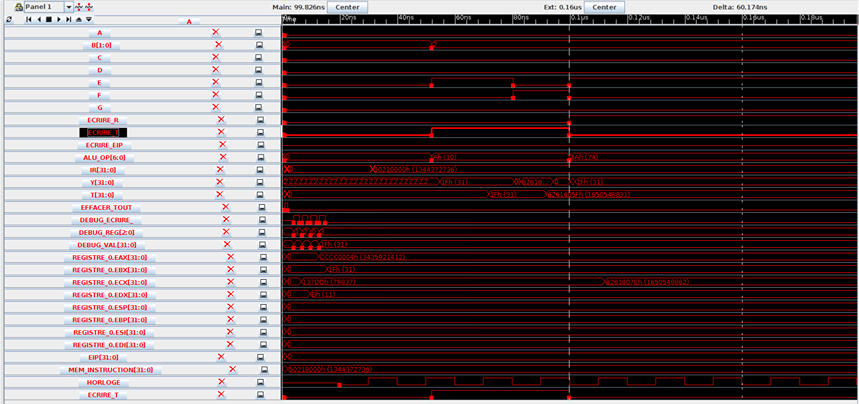
\includegraphics[width=1.7\textwidth]{tp1_ex4_1}}
	\caption{Simulation de $R[1] \leftarrow Mem2[R[3]] + R[3]$}
	\label{}
\end{figure}


\newpage
\begin{enumerate}
	\setcounter{enumi}{1}
	\item
	      \begin{enumerate}[label=\alph*)]
	      	\item en hexadecimal(comme \'ecrit dans le mem1.txt) : 23 80 21 02 \\
	      	      cela donne la valeur : 02 21 80 23\\
	      	      les valeurs ont \'et\'e ecrit comme suit :
	      	      \begin{align*}
	      	      	\underbrace{0000 0010}_{\mbox{Op code}}
	      	      	\underbrace{001}_{\mbox{ecrire R[1]}}
	      	      	\underbrace{010}_{\mbox{lire R[2]}}
	      	      	\underbrace{011}_{\mbox{lire R[3]}}
	      	      	\underbrace{00}_{\mbox{S/O}}
	      	      	\underbrace{0 0000 0010 0011}_{\mbox{op\'erant hex}}
	      	      \end{align*}
	      	\item
	      	      \begin{align*}
	      	      	T \leftarrow R[3];          \\
	      	      	T \leftarrow M2[T];         \\
	      	      	T \leftarrow T + IR<0..12>; \\
	      	      	R[1] \leftarrow T << R[2];  \\
	      	      \end{align*}
	      	\item
	      \end{enumerate}
\end{enumerate}
\begin{figure}[h]
	\begin{tabular}{*{13}{|c} |}
		\hline
		Instruction                  & A & B & C & D & E & F & G & H & UAL & ecrireEIP & ecrireT & ecrireRegistre \\ \hline
		$T \leftarrow R[3]$          & 0 & 2 & 0 & 0 & 1 & 0 & 0 & 0 & 0a  & 0         & 1       & 0              \\ \hline
		$T \leftarrow M2[T]$         & 0 & 2 & 0 & 0 & 0 & 1 & 0 & 0 & 0a  & 0         & 1       & 0              \\ \hline
		$T \leftarrow T + IR<0..12>$ & 0 & 2 & 0 & 1 & 0 & 0 & 0 & 0 & 4a  & 0         & 1       & 0              \\ \hline
		$R[1] \leftarrow T >> R[2]$  & 0 & 1 & 0 & 0 & 1 & 0 & 0 & 0 & 11  & 0         & 0       & 1              \\ \hline
	\end{tabular}
\end{figure}
%ajout du d)
\newpage
\begin{enumerate}
	\begin{enumerate}[label=\alph*)]
		\setcounter{enumii}{3}
		\item
	\end{enumerate}
\end{enumerate}

\begin{figure}[h]
	\makebox[\textwidth][c]{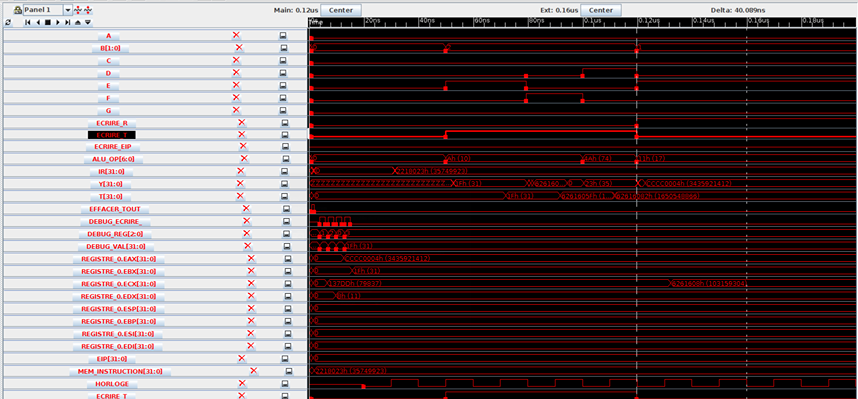
\includegraphics[width=1.7\textwidth]{tp1_ex4_2}}
	\caption{Simulation de $R[1] \leftarrow Mem2[R[3]] + 0x23 << R[2]$}
	\label{}
\end{figure}

\end{document}
